\documentclass[11pt]{article}

\usepackage[
    left=1.0in,
    right=1.0in,
    top=1.0in,
    bottom=1.0in,
    paperwidth=8.5in,
    paperheight=11in,
]{geometry}

%\usepackage[render]{pdf_poker}
\usepackage{pdf_poker}

\usepackage{tabularray}

\begin{document}

\title{pdf\_poker for \LaTeX{}}

\author{Christopher Donham}

\date{March 26, 2025}

\maketitle

\centerline{
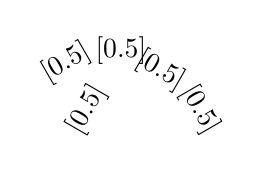
\begin{tikzpicture}
  \node (img1) {\rotatebox{60}{\CardTenClubs[0.5]}};
  \node (img2) at (img1.east) [xshift=-0.7cm, yshift=0.6cm] {\rotatebox{30}{\CardJackDiamonds[0.5]}};
  \node (img3) at (img1.east) [xshift=0cm, yshift=0.75cm] {\CardQueenClubs[0.5]};
  \node (img4) at (img1.east) [xshift=0.5cm, yshift=0.5cm] {\rotatebox{-30}{\CardKingHearts[0.5]}};
  \node (img5) at (img1.east) [xshift=1cm, yshift=0cm] {\rotatebox{-60}{\CardAceSpades[0.5]}};
\end{tikzpicture}}

\section{Introduction}

I am a statistics teacher and use pdflatex with Beamer to create
slides for my lessons.  Playing cards are commonly used to explain
probability, and feature in some of my slides.  A fine library of
playing cards is available in pstricks.  However, Beamer, pdflatex and
pstricks do not interact well.  I also occasionally find other times
when packages I am using in pdflatex do not allow me to use pstricks.
I wrote this package so that I could use playing cards without having
to fight with pstricks.  

Currently, the package provides the 52 that comprise a standard deck
of cards.  There is no provision for drawing the back of a card.
There are currently no jokers or other special cards.

\section{Installation}

The files needed to install this package consist of the the
\textbf{pdf\_poker.sty} file and the files in the \textbf{images
  directory}.  The images are the center portion of the face cards.
There are currently two versions of each image: 1) a tex version that
will render the face card image using tikzpicture, and 2) a png
version that is a pre-rendered image of the face card generated from
the tex version.  Technically, you do not need both version of each
image if you will only be using one of the operating modes of the
package.

\section{Usage}

The default operation of the package uses the pre-rendered versions
of the face cards.  This introduces a dependence on the graphicx
package.  If the drawing of the face card images is insufficient
for your application, then the ``render'' flag will cause the package
to draw all face cards using tikzpicture.

usepackage\[render\]\{pdf\_poker\}

usepackage\{pdf\_poker\}

Each card has an optional scale factor to increase or decrease the size
of the card.

\centerline{\begin{tblr}{width={0.7\linewidth}, colspec={X[c]X[c]X[c]X[c]X[c]}}
Scale = 0.3          & Scale = 0.4          & Scale = 0.5          & Scale = 0.6 & Scale = 0.7 \\
\CardJackHearts[0.3] & \CardJackHearts[0.4] & \CardJackHearts[0.5] & \CardJackHearts[0.6] & \CardJackHearts[0.7] \\
\end{tblr}}

Shown below are the names for all of the cards in the deck.

\centerline{\begin{tblr}{width={0.9\linewidth}, colspec={XXXX}}
CardAceSpades   & CardAceHearts   & CardAceDiamonds   & CardAceClubs \\
CardTwoSpades   & CardTwoHearts   & CardTwoDiamonds   & CardTwoClubs \\
CardThreeSpades & CardThreeHearts & CardThreeDiamonds & CardThreeClubs \\
CardFourSpades  & CardFourHearts  & CardFourDiamonds  & CardFourClubs \\
CardFiveSpades  & CardFiveHearts  & CardFiveDiamonds  & CardFiveClubs \\
CardSixSpades   & CardSixHearts   & CardSixDiamonds   & CardSixClubs \\
CardSevenSpades & CardSevenHearts & CardSevenDiamonds & CardSevenClubs \\
CardEightSpades & CardEightHearts & CardEightDiamonds & CardEightClubs \\
CardNineSpades  & CardNineHearts  & CardNineDiamonds  & CardNineClubs \\
CardTenSpades   & CardTenHearts   & CardTenDiamonds   & CardTenClubs \\
CardJackSpades  & CardJackHearts  & CardJackDiamonds  & CardJackClubs \\
CardQueenSpades & CardQueenHearts & CardQueenDiamonds & CardQueenClubs \\
CardKingSpades  & CardKingHearts  & CardKingDiamonds  & CardKingClubs \\
\end{tblr}}

\section{Requests for Enhancement}

RFE's for the future include:

\begin{itemize}
\item Draw the back of a card.

\item The code is fragile because the symbol for diamonds and hearts
  comes from a different font than the clubs and spades.  Unfortunately,
  the symbols are slightly different sizes resulting in a hard coded
  scale factor.
\end{itemize}  

\CardAceSpades[0.3]
\CardTwoSpades[0.3]
\CardThreeSpades[0.3]
\CardFourSpades[0.3]
\CardFiveSpades[0.3]
\CardSixSpades[0.3]
\CardSevenSpades[0.3]
\CardEightSpades[0.3]
\CardNineSpades[0.3]
\CardTenSpades[0.3]
\CardJackSpades[0.3]
\CardQueenSpades[0.3]
\CardKingSpades[0.3]

\CardAceHearts[0.3]
\CardTwoHearts[0.3]
\CardThreeHearts[0.3]
\CardFourHearts[0.3]
\CardFiveHearts[0.3]
\CardSixHearts[0.3]
\CardSevenHearts[0.3]
\CardEightHearts[0.3]
\CardNineHearts[0.3]
\CardTenHearts[0.3]
\CardJackHearts[0.3]
\CardQueenHearts[0.3]
\CardKingHearts[0.3]

\CardAceDiamonds[0.3]
\CardTwoDiamonds[0.3]
\CardThreeDiamonds[0.3]
\CardFourDiamonds[0.3]
\CardFiveDiamonds[0.3]
\CardSixDiamonds[0.3]
\CardSevenDiamonds[0.3]
\CardEightDiamonds[0.3]
\CardNineDiamonds[0.3]
\CardTenDiamonds[0.3]
\CardJackDiamonds[0.3]
\CardQueenDiamonds[0.3]
\CardKingDiamonds[0.3]

\CardAceClubs[0.3]
\CardTwoClubs[0.3]
\CardThreeClubs[0.3]
\CardFourClubs[0.3]
\CardFiveClubs[0.3]
\CardSixClubs[0.3]
\CardSevenClubs[0.3]
\CardEightClubs[0.3]
\CardNineClubs[0.3]
\CardTenClubs[0.3]
\CardJackClubs[0.3]
\CardQueenClubs[0.3]
\CardKingClubs[0.3]

\end{document}
